\documentclass{ximera}

\usepackage{todonotes}

\newcommand{\RR}{\mathbb R}
\renewcommand{\d}{\,d}
\newcommand{\dd}[2][]{\frac{d #1}{d #2}}
\renewcommand{\l}{\ell}
\newcommand{\ddx}{\frac{d}{dx}}
\newcommand{\dfn}{\textbf}
\newcommand{\eval}[1]{\bigg[ #1 \bigg]}
\renewcommand{\epsilon}{\varepsilon}
\newcommand{\p}[1]{\left(#1\right)}
\newcommand{\br}[1]{\left[#1\right]}
\newcommand{\set}[1]{\left\{#1\right\}}


\let\prelim\lim
\renewcommand{\lim}{\displaystyle\prelim}

\colorlet{textColor}{black} 
\colorlet{background}{white}
\colorlet{penColor}{blue!50!black} % Color of a curve in a plot
\colorlet{penColor2}{red!50!black}% Color of a curve in a plot
\colorlet{penColor3}{red!50!blue} % Color of a curve in a plot
\colorlet{penColor4}{green!50!black} % Color of a curve in a plot
\colorlet{penColor5}{orange!80!black} % Color of a curve in a plot
\colorlet{fill1}{blue!50!black!20} % Color of fill in a plot
\colorlet{fill2}{blue!10} % Color of fill in a plot
\colorlet{fillp}{fill1} % Color of positive area
\colorlet{filln}{red!50!black!20} % Color of negative area
\colorlet{gridColor}{gray!50} % Color of grid in a plot


\newcommand{\fullwidth}{}
\newcommand{\normalwidth}{}



%% makes a snazzy t-chart for evaluating functions
\newenvironment{tchart}{\rowcolors{2}{}{background!90!textColor}\array}{\endarray}


\author{Gregory Hartman \and Matthew Carr}
\license{Creative Commons 3.0 By-NC}
\acknowledgement{https://github.com/APEXCalculus}

\begin{document}
\begin{exercise}

\tag{derivative}


\outcome{Understand the derivative as a function related to the original function.}\outcome{Use the first derivative to determine whether a function is increasing or de- creasing.}

%% BADBAD approximation? Does ximera take plus or minus 1 as an answer? That is, does it take �1?


Using the graph of $g(x)$ shown below, answer the following questions.

\noindent\begin{minipage}[t]{.49\linewidth}
\begin{enumerate}
\item		Where is $g(x) > 0$?
\item		Where is $g(x) < 0$?
\item		Where is $g(x) = 0$?
\end{enumerate}
\end{minipage}
\begin{minipage}[t]{.49\linewidth}
\begin{enumerate}\addtocounter{enumi}{3}
\item		Where is $g'(x) < 0$?
\item		Where is $g'(x) > 0$?
\item		Where is $g'(x) = 0$?
\end{enumerate}
\end{minipage}

\begin{center}
\noindent\begin{minipage}[t]{.5\linewidth}
 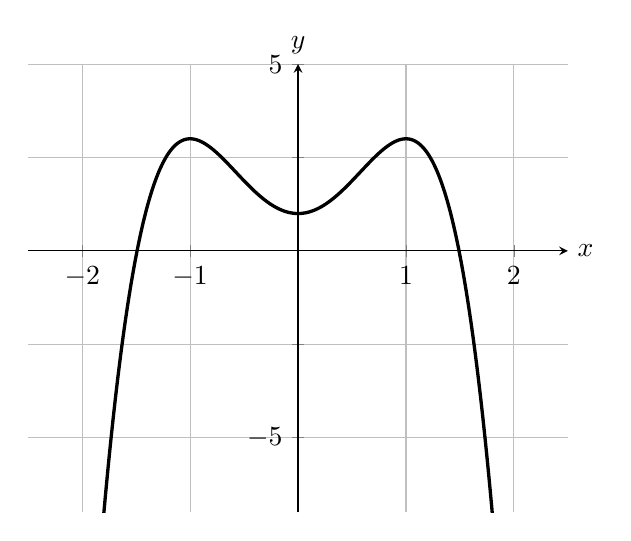
\begin{tikzpicture}
	\begin{axis}
	[ymin=-7,ymax=5, xmin=-2.5,xmax=2.5, axis lines=center,xlabel=$x$,ylabel=$y$,every axis y 
	label/.style={at=(current axis.above origin),anchor=south},every axis x label/.style={at=(current axis.right of origin),anchor=west},
	domain=-3:3,
	ytick={-5,-2.5,0,2.5,5},
	yticklabels={$-5$,,,,$5$},
	xtick={-2,-1,1,2},
	xticklabels={$-2$,$-1$,$1$,$2$},
	ymajorgrids=true,
	grid = major
	]
	\addplot[domain=-2:2,very thick,smooth,samples=1000]
	{4*pow(\x,2)-2*pow(\x,4)+1};
	\end{axis}
       \end{tikzpicture}
\end{minipage}
\end{center}

\noindent\begin{minipage}[t]{.49\linewidth}
\begin{enumerate}
\item		On $\begin{prompt}\answer{(-1.5,1.5)}\end{prompt}$
\item		On $\begin{prompt}\answer{(-\infty,-1.5) \cup (1.5,\infty)}\end{prompt}$
\item		At $x\begin{prompt} = \answer{\pm1.5}\end{prompt}$
\end{enumerate}
\end{minipage}
\begin{minipage}[t]{.49\linewidth}
\begin{enumerate}\addtocounter{enumi}{3}
\item		On $\begin{prompt}\answer{(-\infty,-1)\cup(0,1)}\end{prompt}$
\item		On $\begin{prompt}\answer{(-1,0)\cup(1,\infty)}\end{prompt}$
\item		At $x\begin{prompt} = \answer{\pm1}\end{prompt}$
\end{enumerate}
\end{minipage}

\end{exercise}
\end{document}